\documentclass[a4paper,10pt]{article} \usepackage{anysize}
\marginsize{2cm}{2cm}{1cm}{1cm}
%\textwidth 6.0in \textheight = 664pt
\usepackage{xunicode} 
\usepackage{xltxtra} 
\usepackage{graphicx}
\usepackage{color} 
\usepackage[EU1]{fontenc}
\usepackage{xgreek} 
\usepackage{fancyvrb}
\usepackage{enumitem} 
\usepackage{framed} 
\usepackage{relsize}
\usepackage{float} 
\setmainfont[Mapping=TeX-text]{Times New Roman}
\renewcommand{\nobreakspace}{\nobreak\ }

\begin{document}

\begin{titlepage}
\begin{center}
\begin{figure}[t] 
     
\includegraphics[scale=0.7]{title/ntua_logo}
\end{figure}
\begin{LARGE}\textbf{ΕΘΝΙΚΟ ΜΕΤΣΟΒΙΟ ΠΟΛΥΤΕΧΝΕΙΟ\\}\end{LARGE}
\vspace{2cm}
\begin{Large}
ΣΧΟΛΗ ΗΜ\&ΜΥ\\
ΣΗΜΑΤΑ ΚΑΙ ΣΥΣΤΗΜΑΤΑ\\
Ακ. έτος 2010-2011\\
ΕΡΓΑΣΙΑ MATLAB\\
\end{Large}
\vspace{5cm}
\vspace{1cm}
\begin{tabular}{l r}
\Large{Λύρας Γρηγόρης}&
\large{Α.Μ.: 03109687}\\
\end{tabular}\\
\vspace{5cm}

\vfill
\large\today\\
\end{center}
\end{titlepage}



\section*{Μέρος $1^o$ - Φασματική Ανάλυση και Ανίχνευση Ημιτονοειδών Σημάτων
με το Διακριτό Μετ/σμό Fourier (DTF)}
\setcounter{section}{1}
Ορίζουμε το σήμα μας ως άθροισμα δύο ημιτόνων διαφορετικών συχνοτήτων σύμφωνα
με τις παρακάτω εξισώσεις.
\begin{equation}
x[n]=[A_1*cos(\Omega_1*n)+A_2*cos(\Omega_2*n)]*w[n]
\end{equation}
\begin{equation}
A_1=1 , A_2=0.75
\end{equation}
\begin{equation}
\Omega_1=pi*mod(\frac{10*max(8,5)}{11*(8+5)},1) 
\end{equation}
\begin{equation}
\Omega_2=mod(\Omega_1=\frac{pi}{4},pi)
\end{equation}

Επίσης το παράθυρο $w[n]$ είναι μοναδιαίο μήκους $L=512$.
\begin{equation}
w[n]=\left\{\begin{array}{l l}
1 & 1 \leq n \leq L-1 \\
0 & else \\
\end{array}
\right.
\end{equation}
\subsection{Αυτοσυσχέτιση}


\begin{figure}[H]
\caption{Αυτοσυσχέτιση}
\centering
	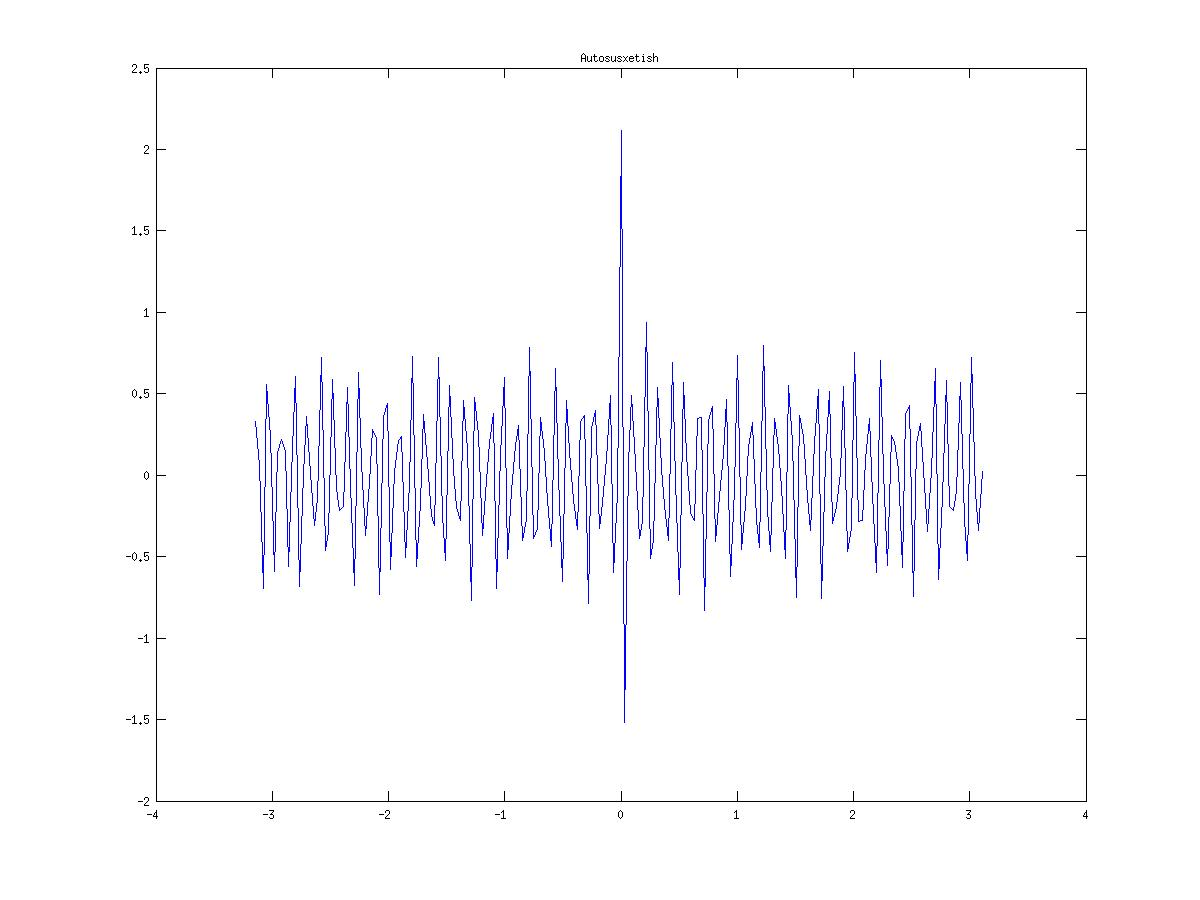
\includegraphics[scale=0.4]{files/01-Autosusxetish.jpg}
\end{figure}
Από το Σχήμα 1 μπορούμε να συμπεράνουμε πως το αρχικό σήμα μας είναι επίσης
περιοδικό και μάλιστα αυτό έχει ίδια περίοδο με αυτή της αυτοσυσχέτισης. Ακόμη
αν πάρουμε το μετασχηματισμό Fourier της αυτοσυσχέτισης αυτός είναι ίσος με το
φάσμα της ισχύος του σήματος. Έτσι μπορούμε να βρούμε τις συχνότητες όπου το
σήμα έχει την μεγαλύτερη ισχύ (δηλαδή τις αρμονικές συνιστώσες του, δύο για το
δοθέν σήμα).

\subsection{DTFT του σήματος 256 δείγματα}
\begin{figure}[H]
\caption{Πλάτος του DTFT με 256 δείγματα}
\centering
	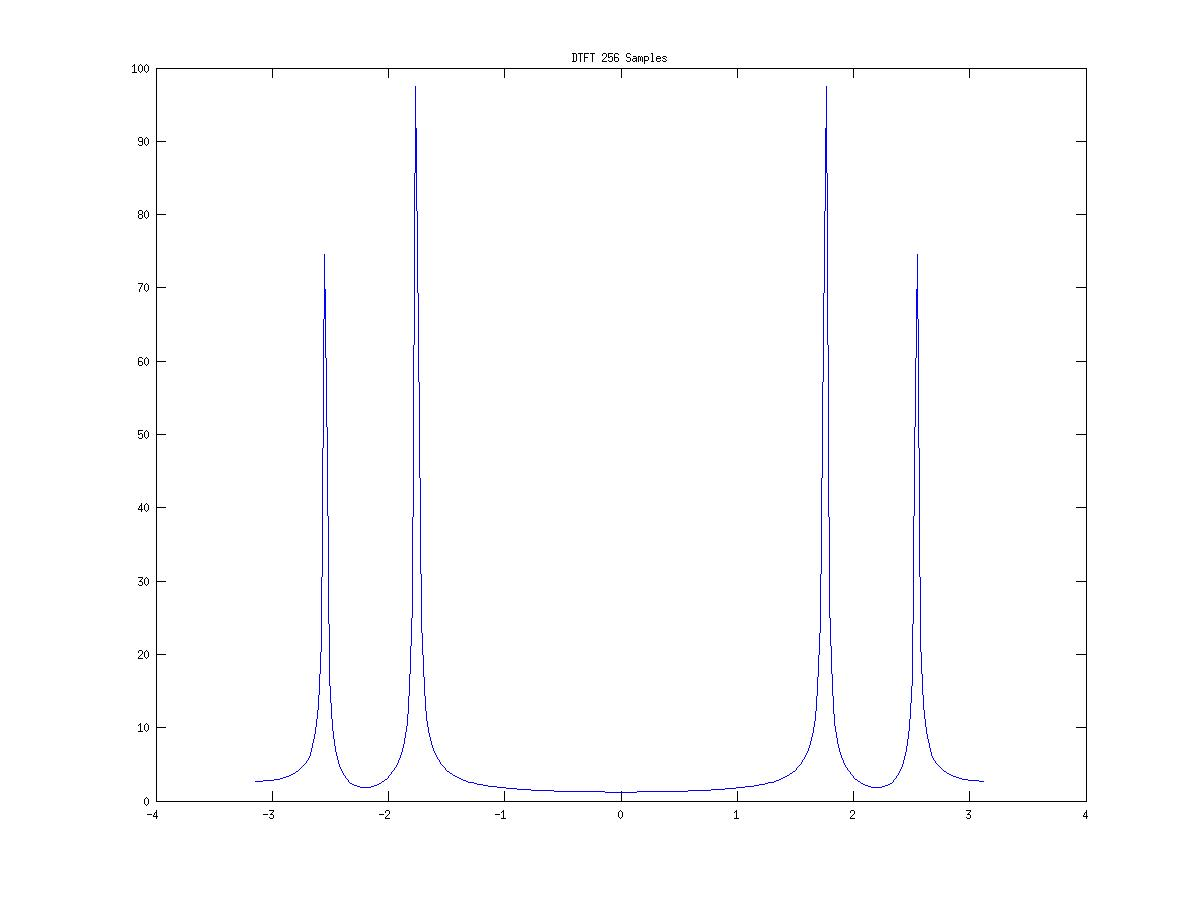
\includegraphics[scale=0.4]{files/02-DTFT_256_Samples.jpg}
\end{figure}
Στο παραπάνω Σχήμα έχουμε τον διακριτό μετασχηματισμό Fourier του αρχικού
σήματος μήκους 256 δειγμάτων. Παρατηρούμε τις δυο συχνότητες που εμφανίζονται
στο σχήμα. Τα μέγιστα βρίσκονται στις συχνότητες $\Omega_1$ και $\Omega_2$
αντίστοιχα.

\subsection{DTFT του σήματος με 256 δείγματα και με μεταβολή των συχνοτήτων}
\begin{figure}[H]
\caption{Πλάτος του DTFT με 256 δείγματα και με μεταβολή των συχνοτήτων}
\centering
	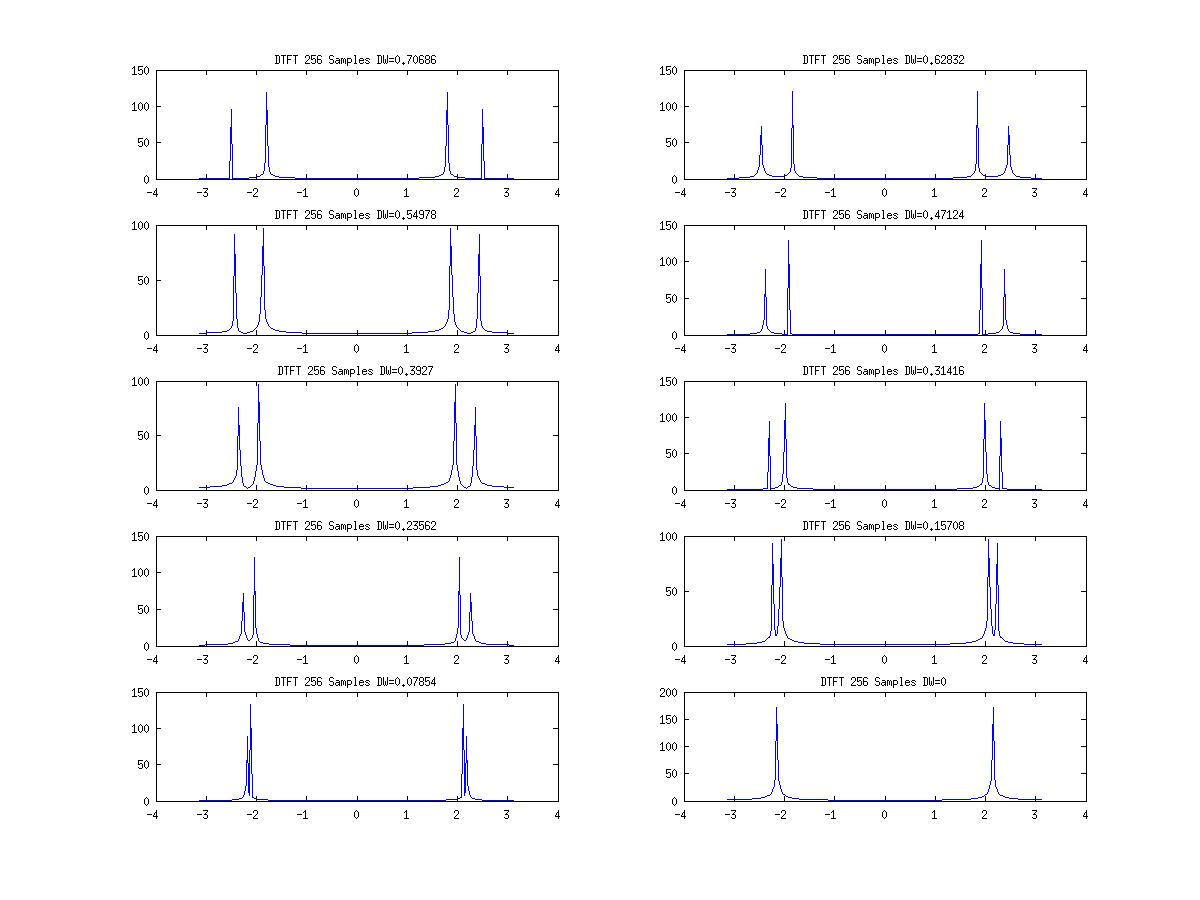
\includegraphics[scale=0.4]{files/03-DTFT_256_Samples.jpg}
\end{figure}
Μεταβάλλουμε τις συχνότητες προς τη μέση τιμή τους. Η διαφορά τους φαίνεται
στο διάγραμμα (DW). Παρατηρούμαι φαινόμενο aliasing από την αρχή συνεπώς
χρειαζόμαστε περισσότερα δείγματα για να ανακατασκευάσουμε το σήμα πλήρως.
\subsection{DTFT του σήματος με περισσότερα δείγματα και με μεταβολή των συχνοτήτων}
\begin{figure}[H]
\caption{Πλάτος του DTFT με 512 δείγματα και με μεταβολή των συχνοτήτων}
\centering
	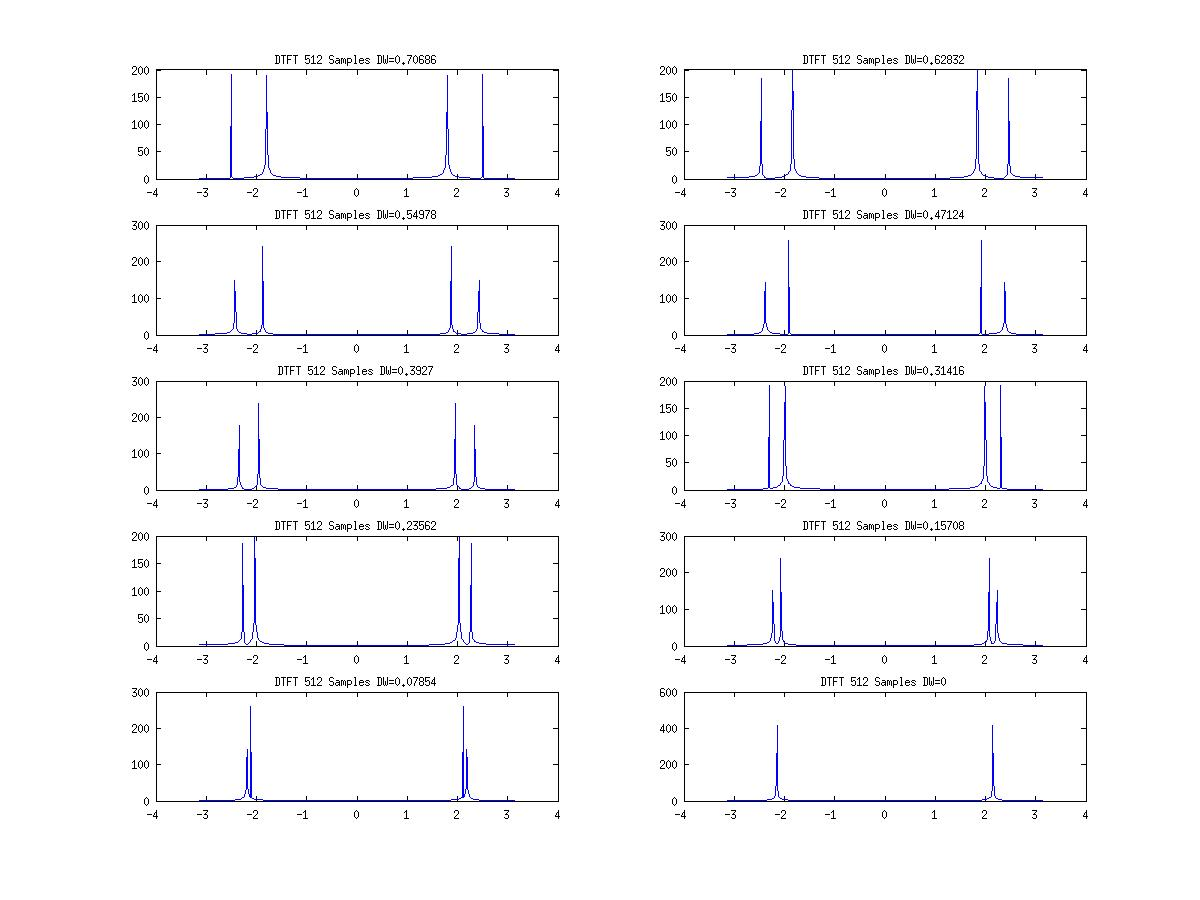
\includegraphics[scale=0.4]{files/04-DTFT_512_Samples.jpg}
\end{figure}
Με 512 δείγματα έχουμε καλύτερη ευκρίνεια στα διαγράμματα και οι συχνότητες
ξεχωρίζουν σαφώς μέχρι η διαφορά των συχνοτήτων φτάσει στα $0.39 rad$
\begin{figure}[H]
\caption{Πλάτος του DTFT με 1024 δείγματα και με μεταβολή των συχνοτήτων}
\centering
	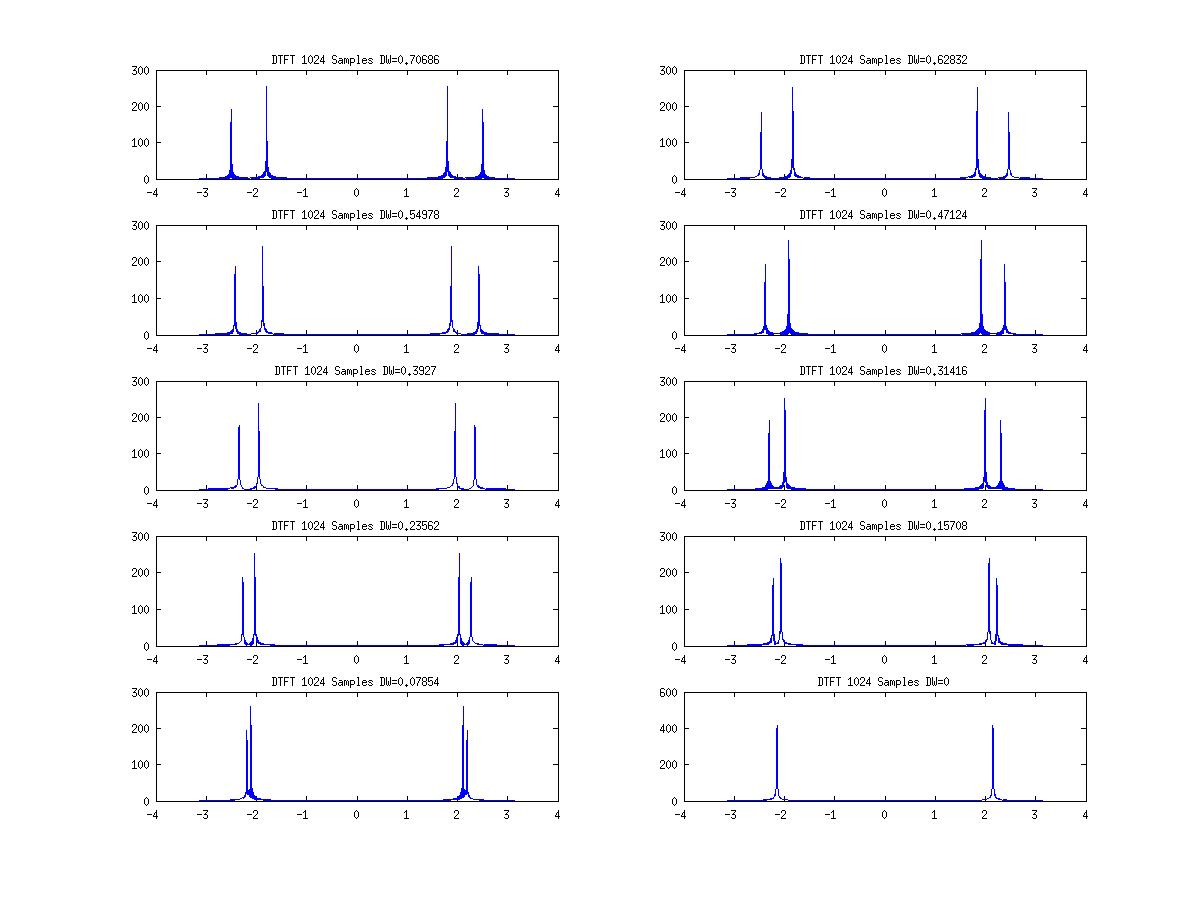
\includegraphics[scale=0.4]{files/05-DTFT_1024_Samples.jpg}
\end{figure}
Αυξάνουμε ακόμη περισσότερο τον αριθμό των δειγμάτων και προσθέτουμε μηδενικά
στο τέλος του σήματος (zero-padding). Αυτό μας δίνει ακόμη καλύτερη εικονα και
όμως στο συγκεκριμένο σήμα η ελάχιστη διαφορά που μπορούμε να διακρίνουμε
είναι πάλι $DW=0.39 rad$ 


\pagebreak
\subsection{Χρήση παραθύρου Hamming}
\begin{equation}
w[n]=\left\{\begin{array}{l l}
0.54 - 0.46*cos(2*pi*\frac{n}{L}) & 1 \leq n \leq L-1 \\
0 & else \\
\end{array}
\right.
\end{equation}



\begin{figure}[H]
\caption{Αυτοσυσχέτιση}
\centering
	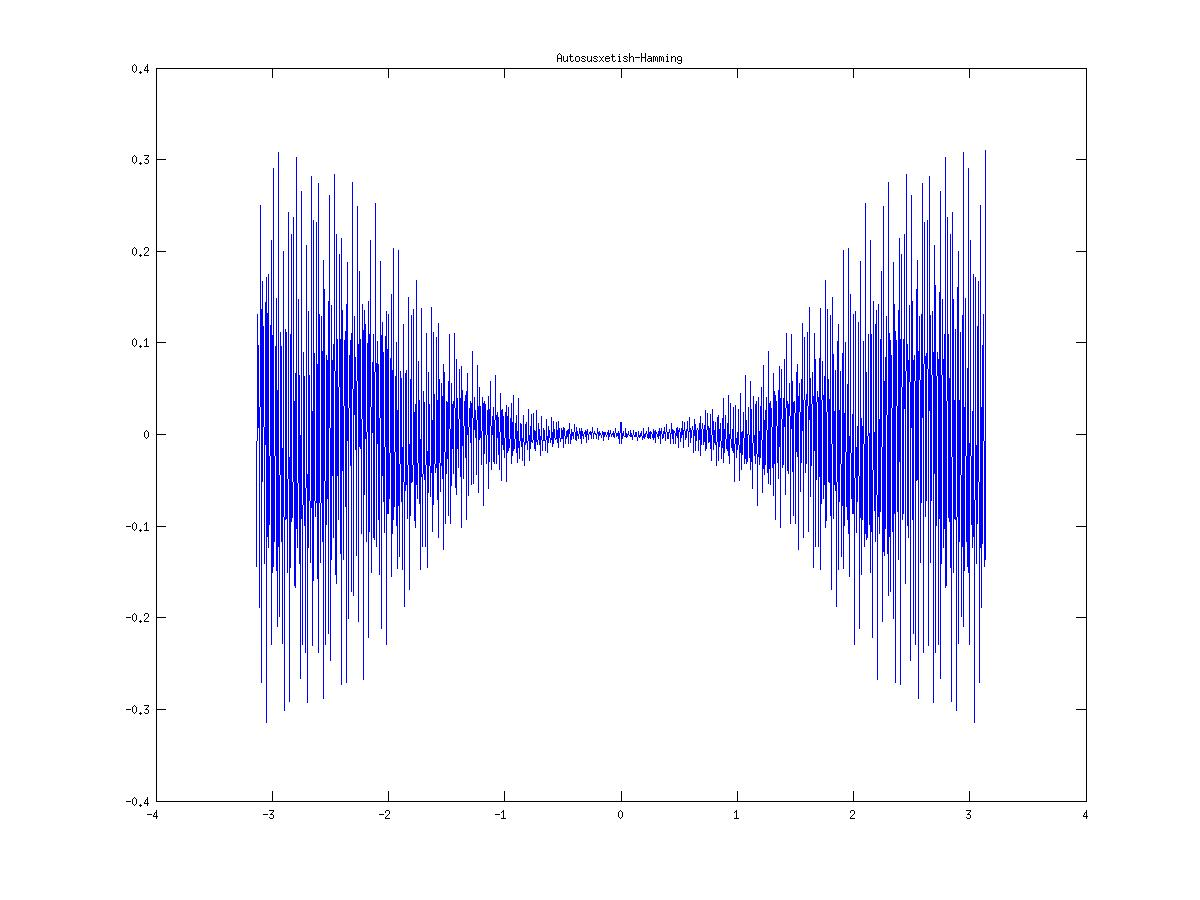
\includegraphics[scale=0.4]{files/11-Autosusxetish-Hamming.jpg}
\end{figure}

\begin{figure}[H]
\caption{Πλάτος του DTFT με 256 δείγματα}
\centering
	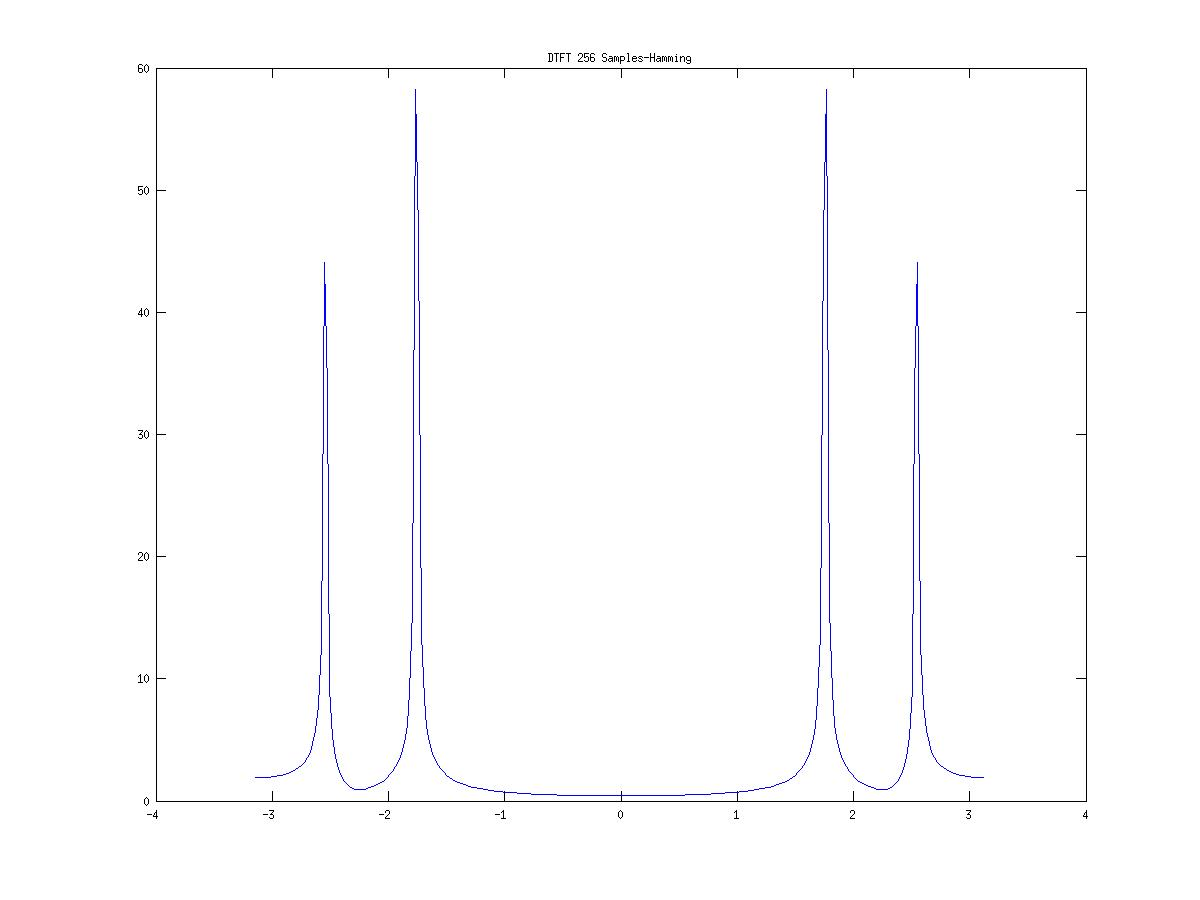
\includegraphics[scale=0.4]{files/12-DTFT_256_Samples-Hamming.jpg}
\end{figure}
\begin{figure}[H]
\caption{Πλάτος του DTFT με 256 δείγματα και με μεταβολή των συχνοτήτων}
\centering
	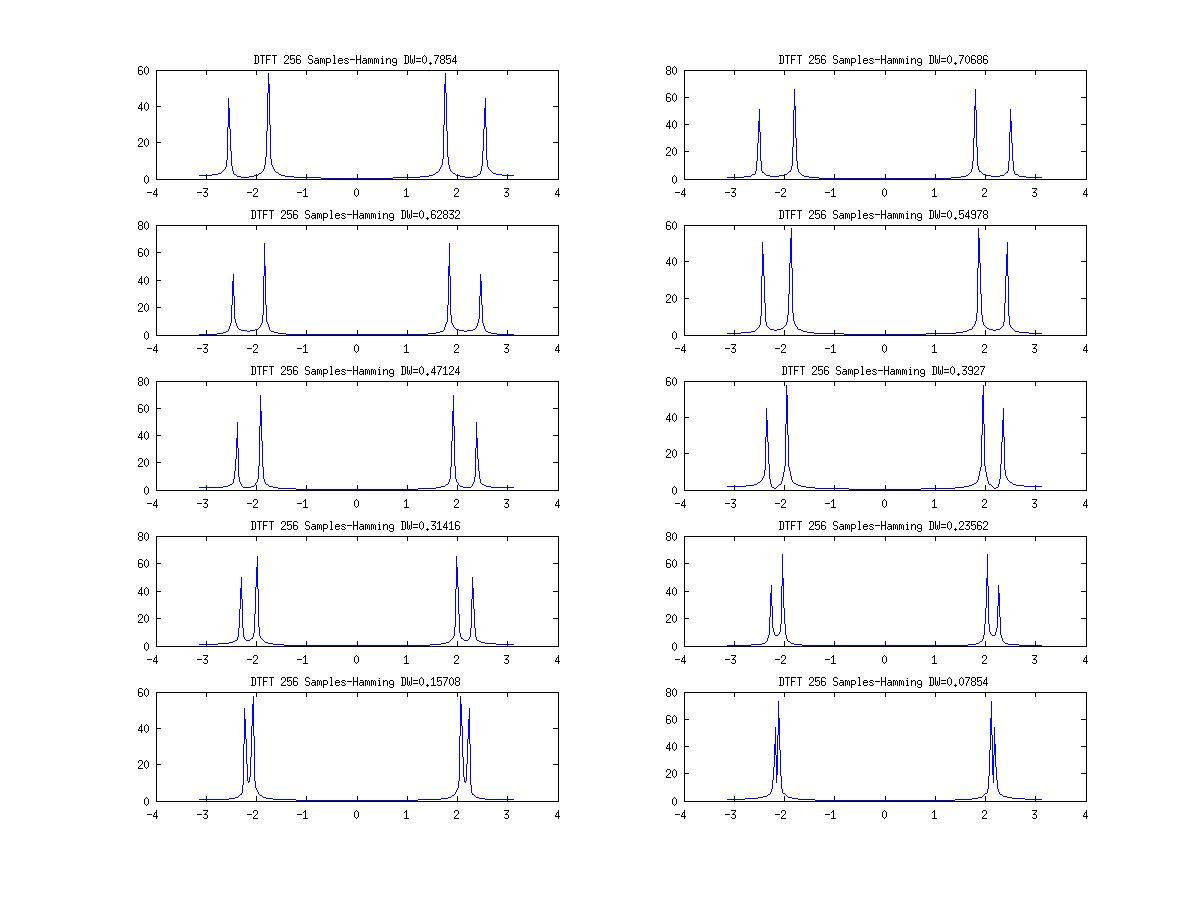
\includegraphics[scale=0.4]{files/13-DTFT_256_Samples-Hamming.jpg}
\end{figure}
Πάλι παρατηρούμε φαινόμενο aliasing συνεπώς πρέπει να αυξήσουμε τον αριθμό των
δειγμάτων.
\begin{figure}[H]
\caption{Πλάτος του DTFT με 512 δείγματα και με μεταβολή των συχνοτήτων}
\centering
	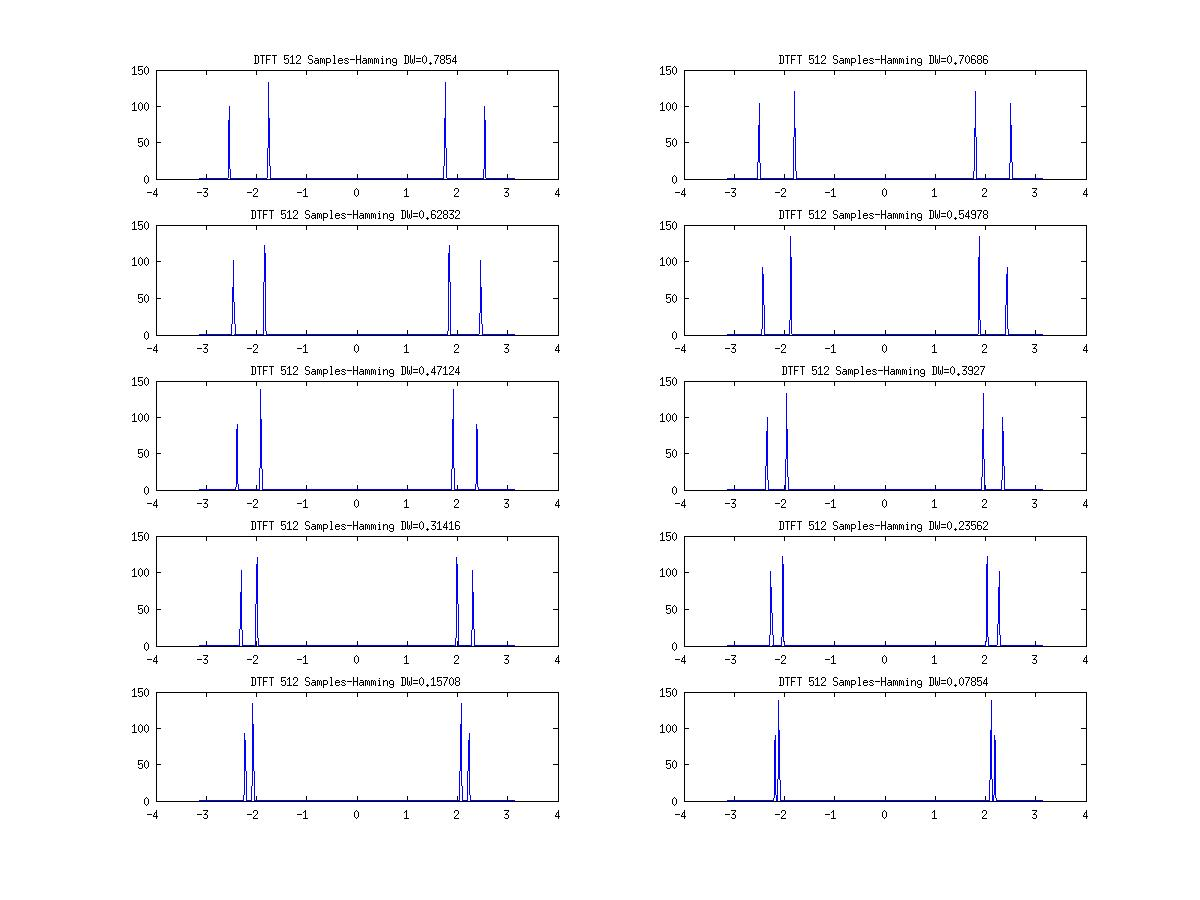
\includegraphics[scale=0.4]{files/14-DTFT_512_Samples-Hamming.jpg}
\end{figure}
Εδώ έχουμε πολύ καθαρότερα διαγράμματα και φτάνουμε να διακρίνουμε διαφορά
συχνοτήτων έως και $DW=0.17rad$.
\begin{figure}[H]
\caption{Πλάτος του DTFT με 1024 δείγματα και με μεταβολή των συχνοτήτων}
\centering
	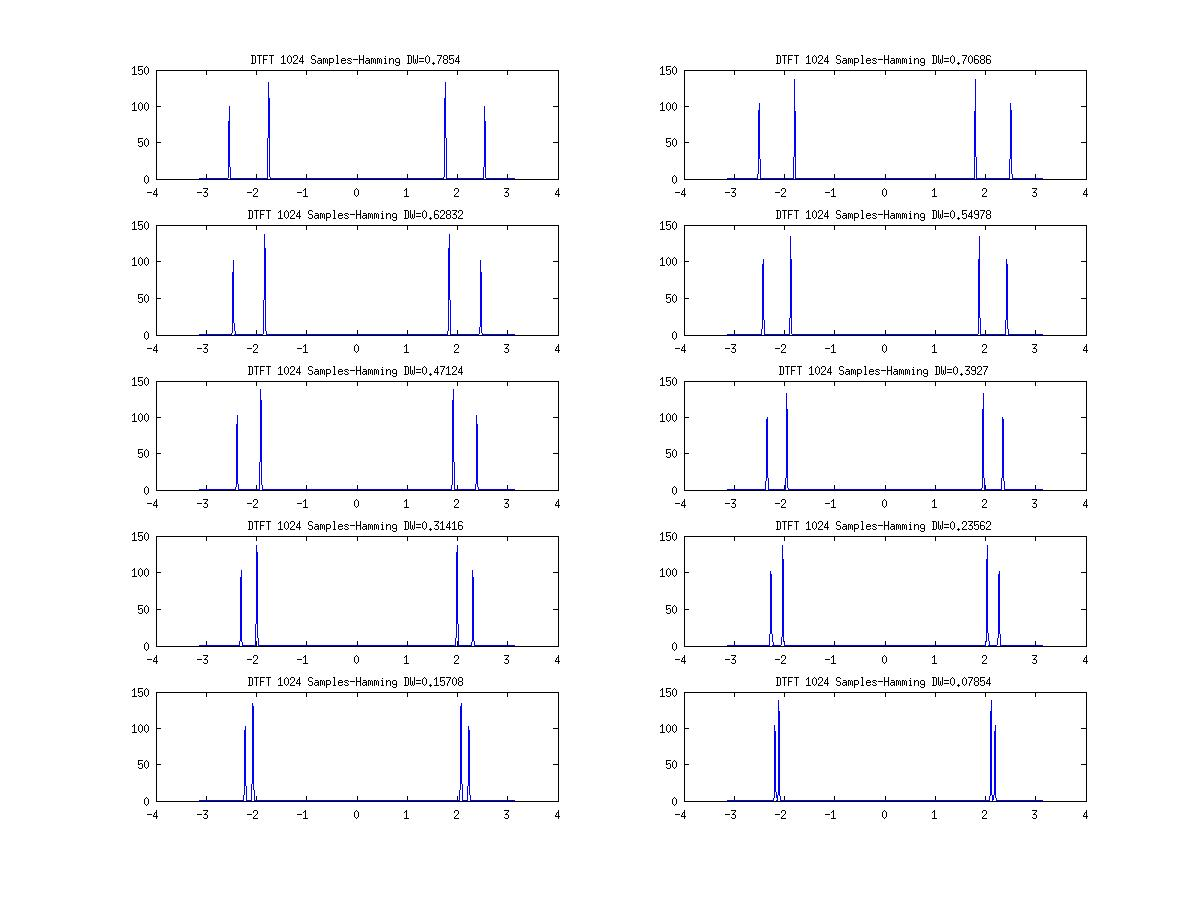
\includegraphics[scale=0.4]{files/15-DTFT_1024_Samples-Hamming.jpg}
\end{figure}
Τέλος φτάνουμε να μπορούμε να διακρίνουμε συχνότητες που διαφέρουν μέχρι και
$DW=0.07rad$.


\pagebreak
\section*{Μέρος $2^o$ - Απόκριση Συστημάτων}


Από το διάγραμμα των πόλων και των μηδενικών ορίσαμε αυθαίρετα τις σχετικές
θέσεις των πόλων και των μηδενικών. Συγκεκριμένα ορίσαμε τον πίνακα των πόλων
και τον πίνακα των μηδενικών:

\begin{figure}[H]
\begin{tabular}{r r}
Πίνακας πόλων & Πίνακας μηδενικών \\
0.8+0.3i &0.6+1.4i\\
0.8-0.3i &0.6-1.4i\\
-0.6+0.4i &\\
-0.6-0.4i &\\
0.3+0.7i &\\
0.3-0.7i &\\
\end{tabular}
\end{figure}
\begin{figure}[H]
\caption{Z-plane}
\centering
	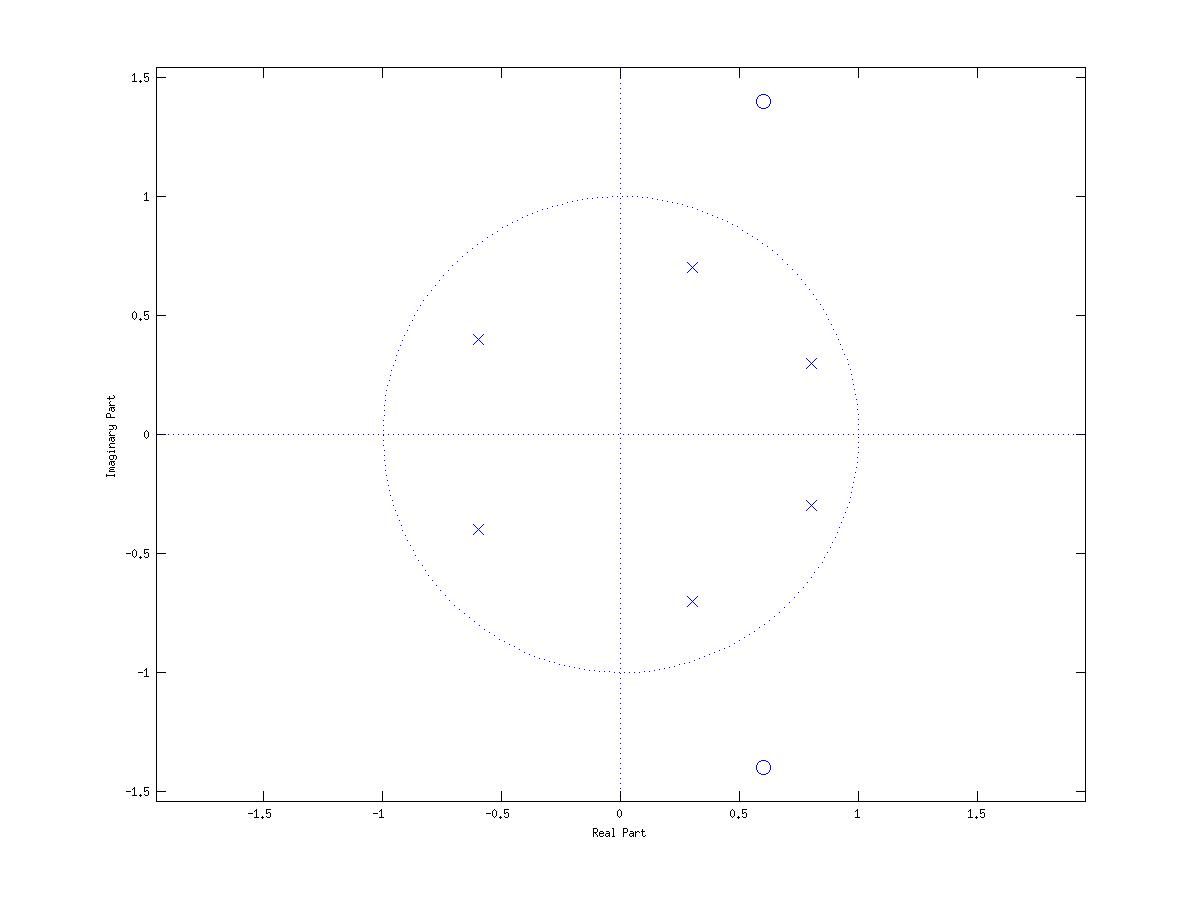
\includegraphics[scale=0.4]{files/21-Z-PLANE.jpg}
\end{figure}







\begin{figure}[H]
\caption{Κρουστική Απόκριση}
\centering
	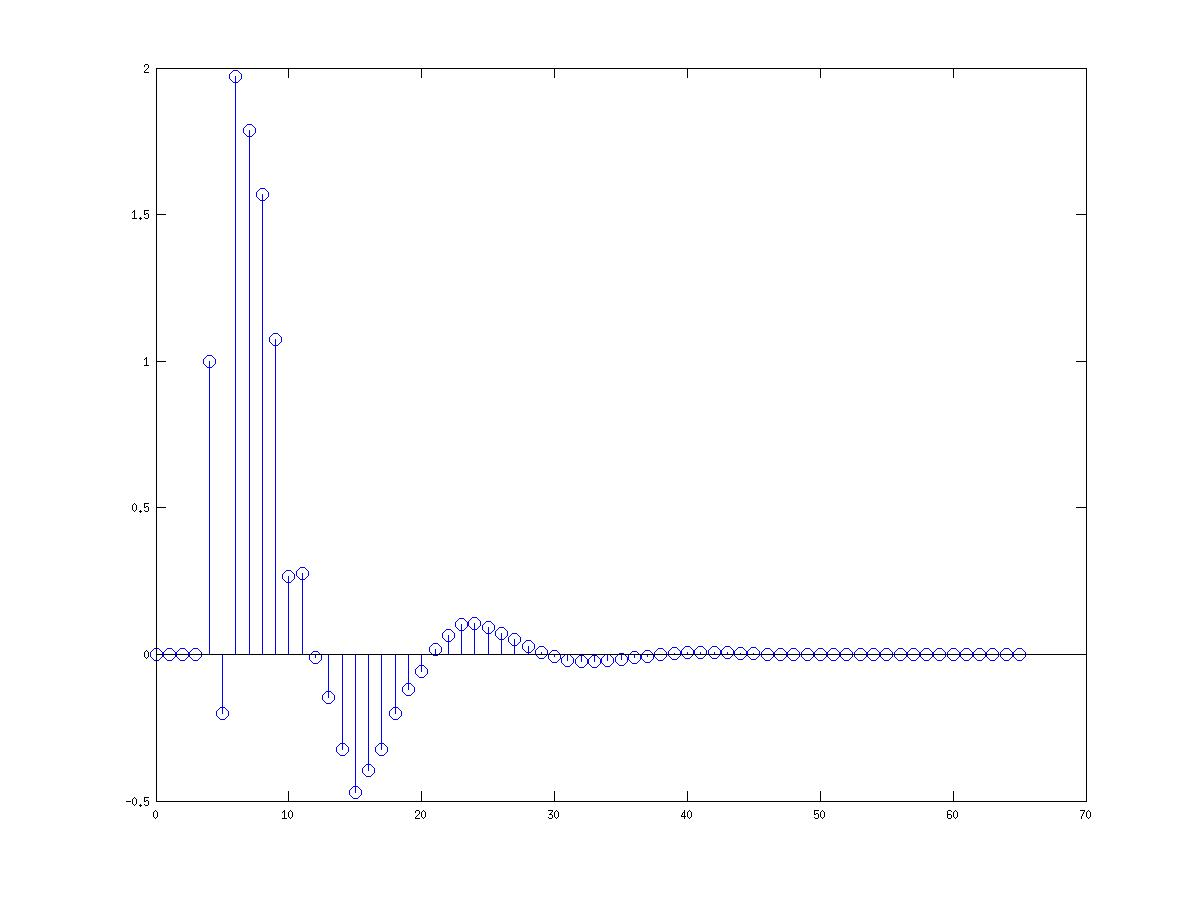
\includegraphics[scale=0.4]{files/21-kroustikh_apokrish.jpg}
\end{figure}



\begin{figure}[H]
\caption{Βηματική Απόκριση}
\centering
	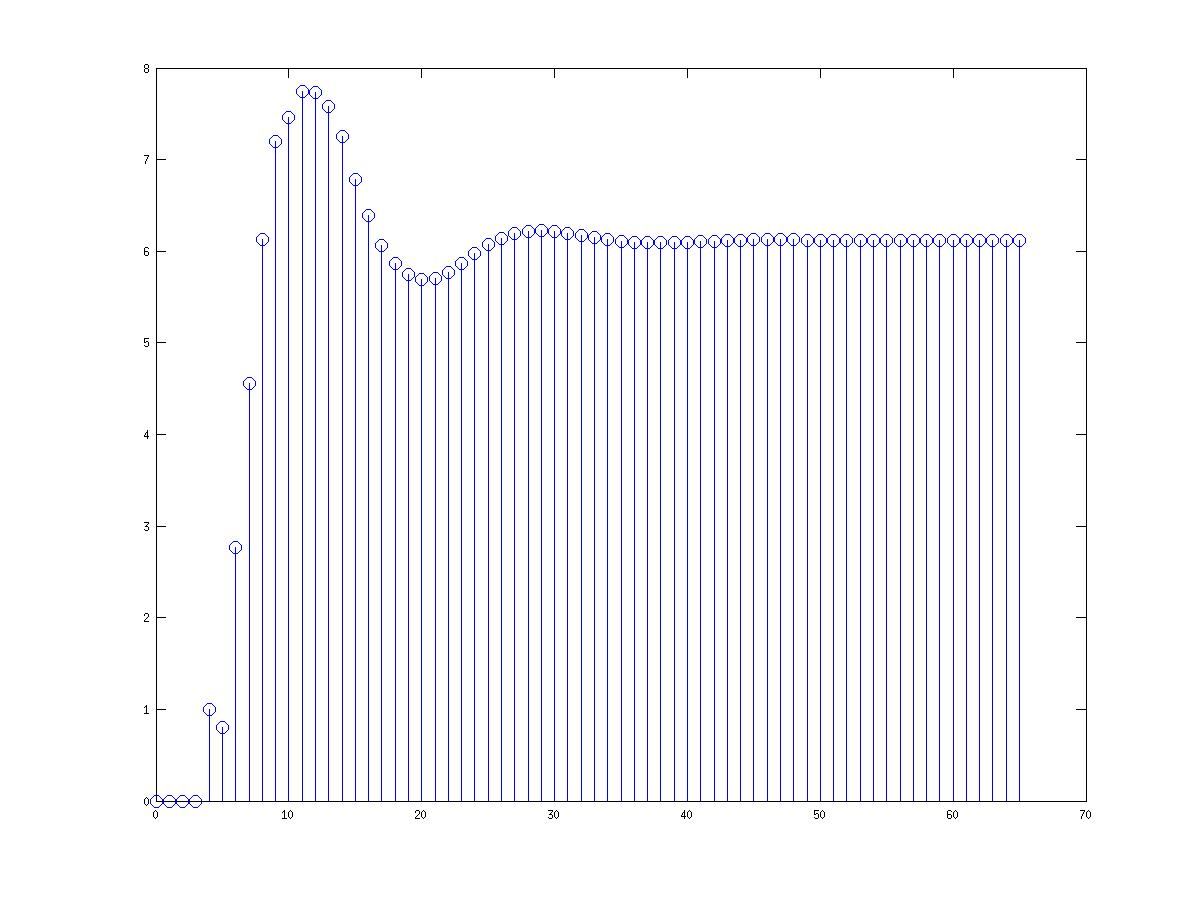
\includegraphics[scale=0.4]{files/22-bhmatikh_apokrish.jpg}
\end{figure}

\begin{figure}[H]
\caption{Απόκριση Πλάτους}
\centering
	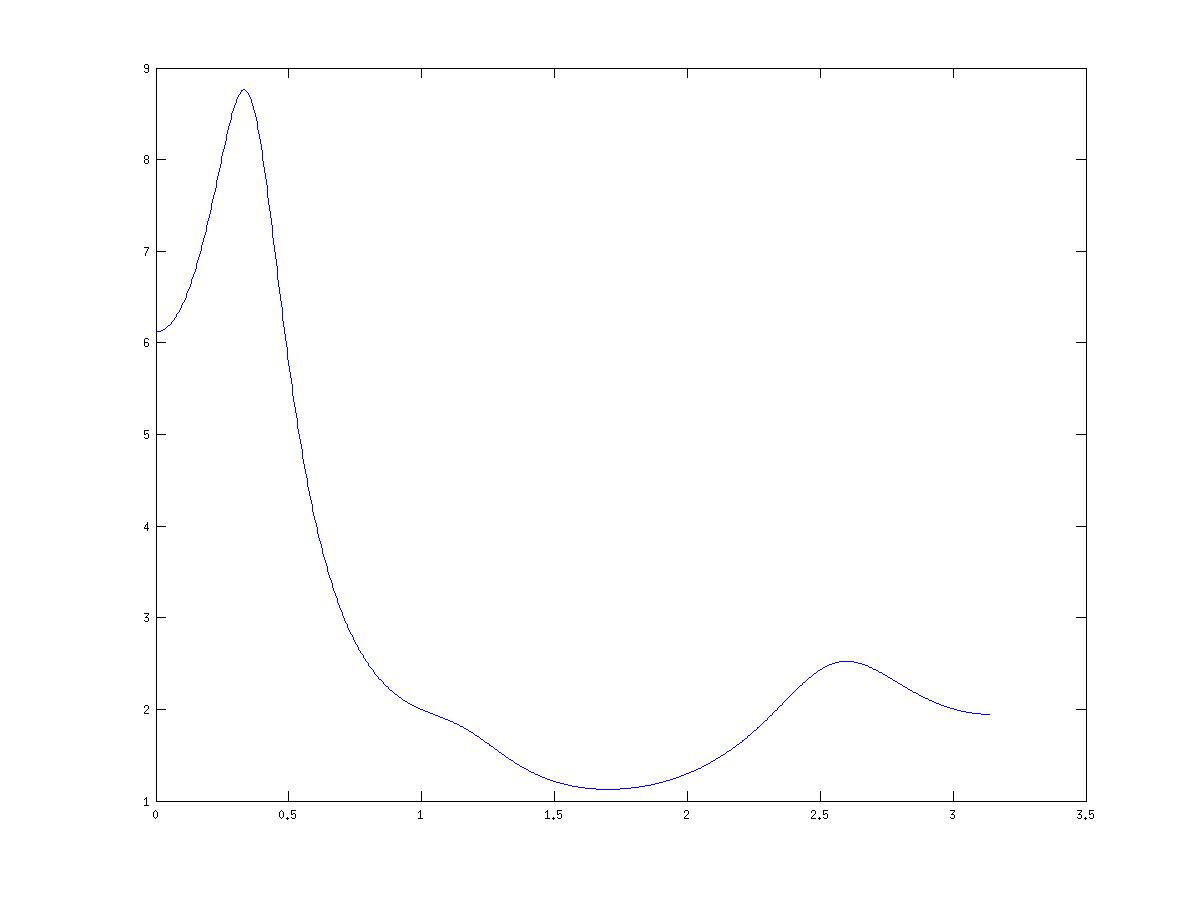
\includegraphics[scale=0.4]{files/23-apokrish_platous.jpg}
\end{figure}

\begin{figure}[H]
\caption{Διέγερση με τυχαίο σήμα}
\centering
	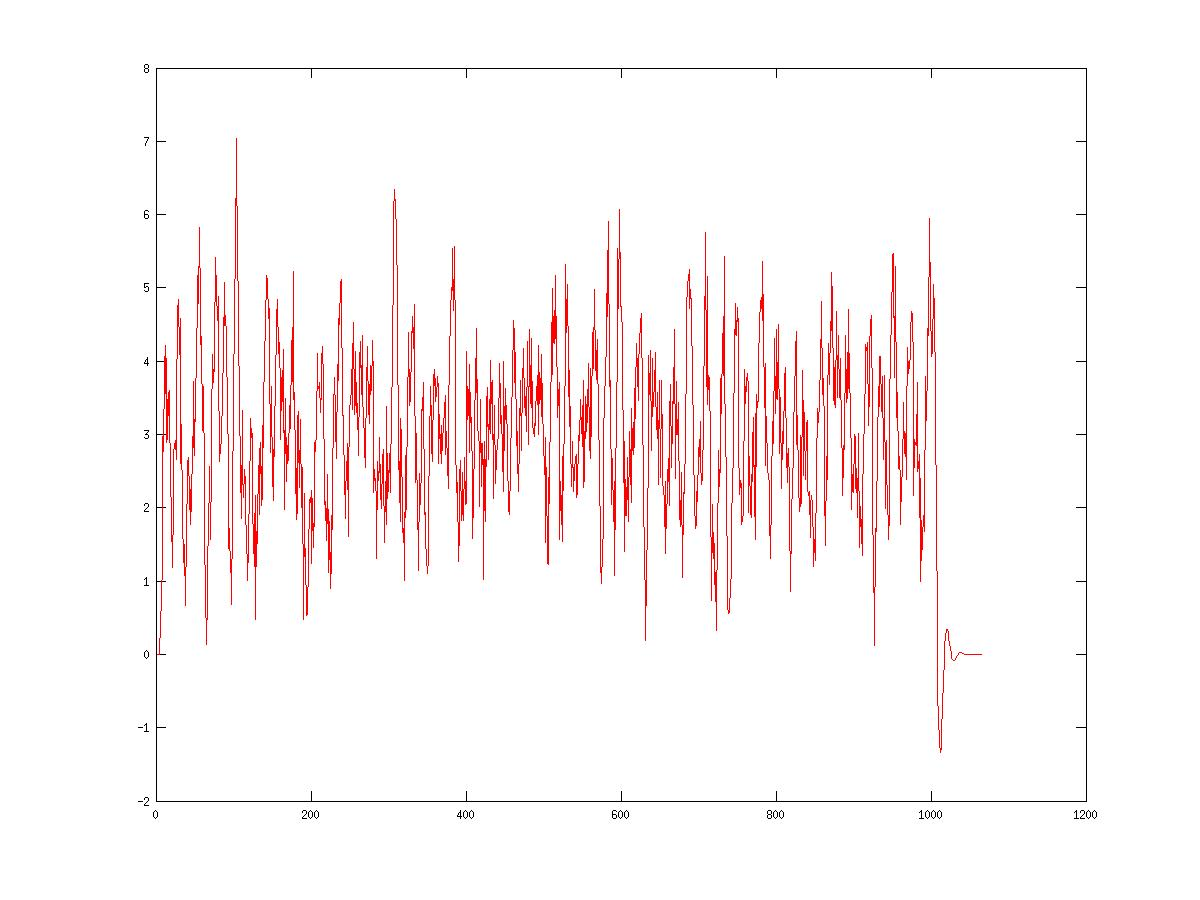
\includegraphics[scale=0.4]{files/24-diegersh_me_tuxaio_shma.jpg}
\end{figure}
 Όταν η είσοδος του συστήματος είναι τυχαίο σήμα τότε η έξοδος του συστήματος
 είναι επίσης τυχαία.

\begin{figure}[H]
\caption{Διέγερση με παλμοσειρά}
\centering
	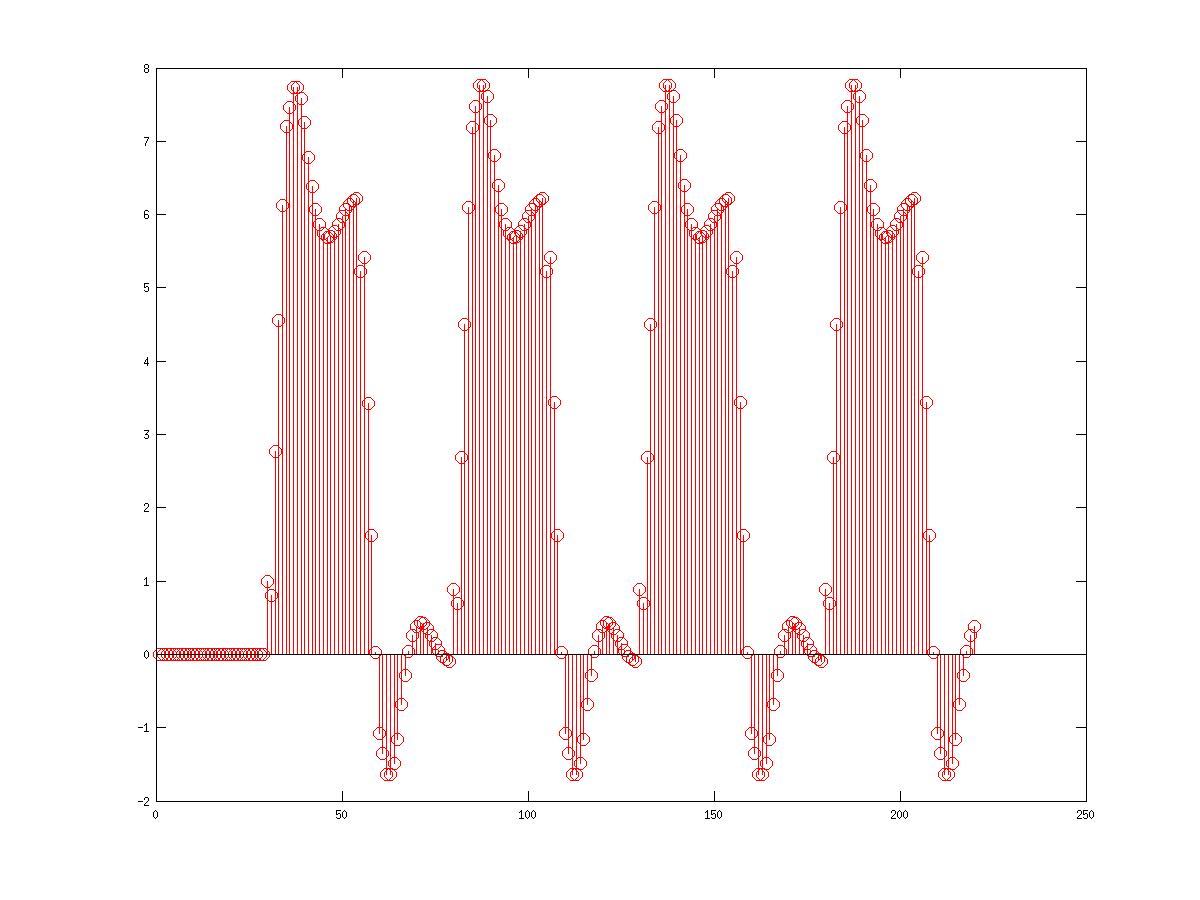
\includegraphics[scale=0.4]{files/25-diegersh_me_palmoseira.jpg}
\end{figure}
Διεγείρουμε το σύστημα με παλμοσειρά. Εμφανίζεται η αρχική εικόνα της
βηματικής απόκρισης σε κάθε παλμό και ή έξοδος είναι περιοδική.

\begin{figure}[H]
\caption{Μετακίνηση πόλων}
\centering
	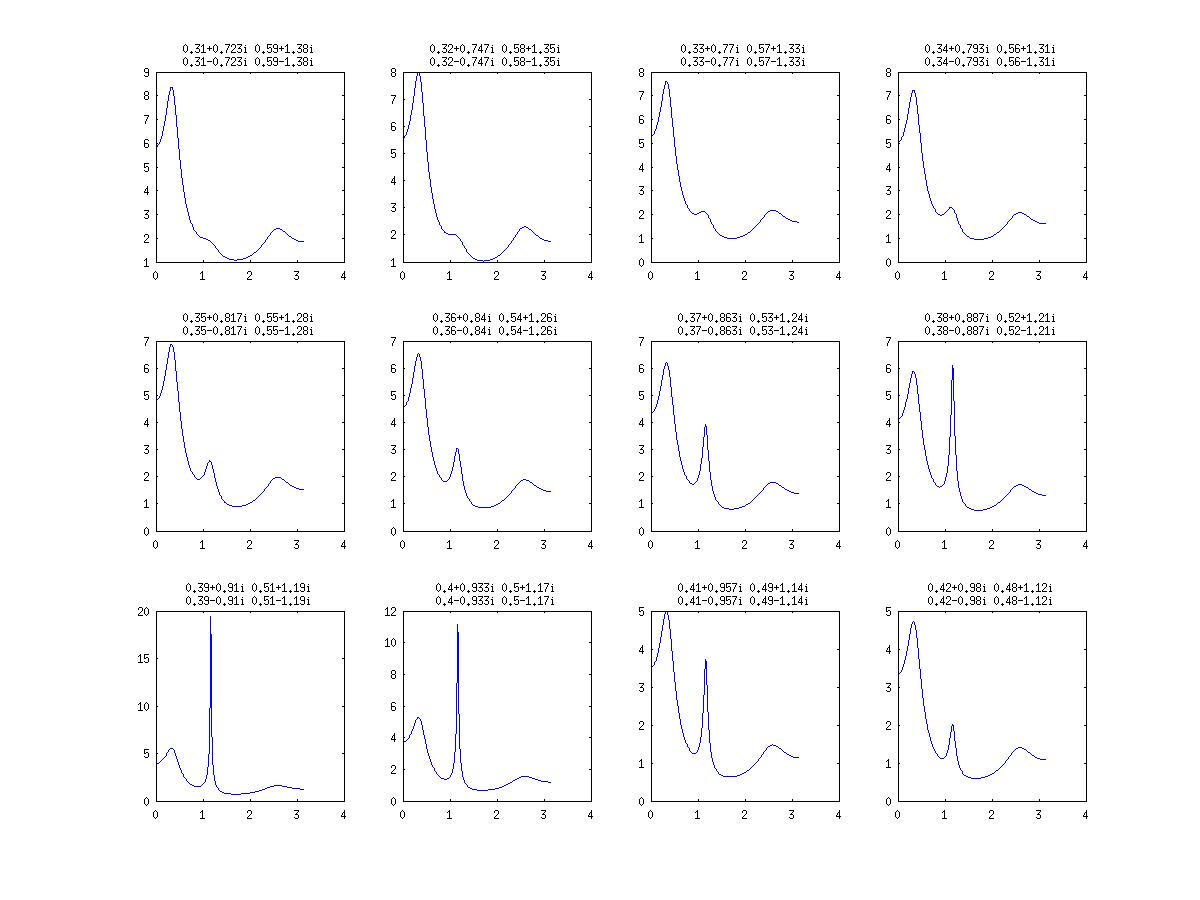
\includegraphics[scale=0.4]{files/26-metakinoumenoi_poloi.jpg}
\end{figure}
Μετακινώντας τους πόλους που βρίσκονται στην ίδια ευθεία με τα μηδενικά
παρατηρούμε πως όσο οι πόλοι πλησιάζουν το μοναδιαίο κύκλο τόσο πιο ασταθές
γίνεται το σύστημα μας όπως φαίνεται και από τα διαδοχικά διαγράμματα
απόκρισης πλάτους. Όταν οι πόλοι συμπέσουν με τα μηδενικά τότε απαλείφονται
και το διάγραμμα απόκρισης πλάτους γίνεται πάλι ομαλό όπως φαίνεται στο
παρακάτω σχήμα. 
\begin{figure}[H]
\caption{Μετακίνηση πόλων (τα μηδενικά και οι πόλοι συμπέφτουν)}
\centering
	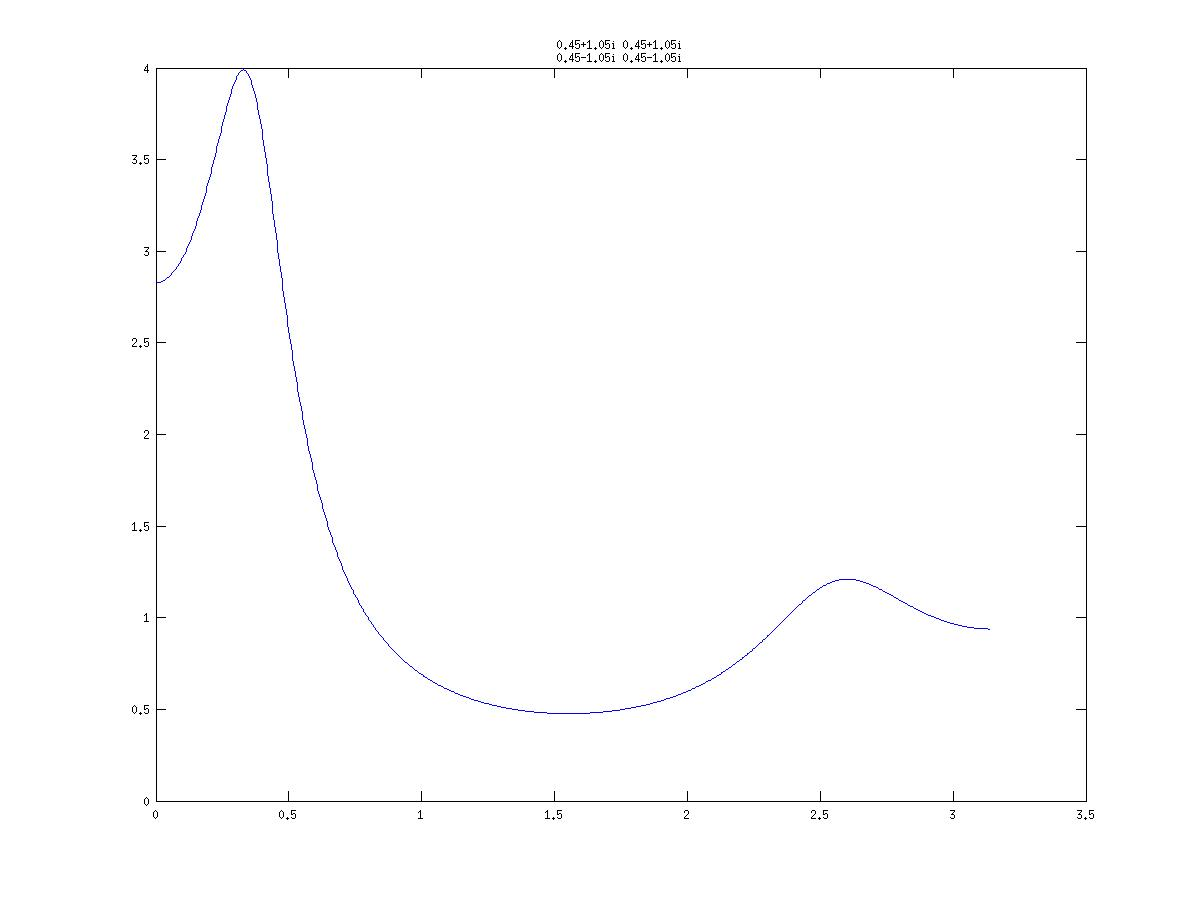
\includegraphics[scale=0.4]{files/26-metakinoumenoi_poloi_last_frame.jpg}
\end{figure}

\end{document}
